\chapter{Panel użytkownika zarejestrowanego}

\section{Logowanie do panelu użytkownika}
W poniższej sekcji przedstawiony zostanie proces logowania do panelu użytkownika w~ aplikacji. W pierwszej kolejności użytkownik musi wybrać opcję \textit{Rozpocznij}, dostępną z~ poziomu górnego menu na stronie głównej, a następnie wpisać login i hasło, bądź wybrać przycisk \textit{Zaloguj się z~ Google}. Okno logowania przedstawione jest na rysunku \ref{Rys:logowanie}.

\begin{figure}[h]
	\centering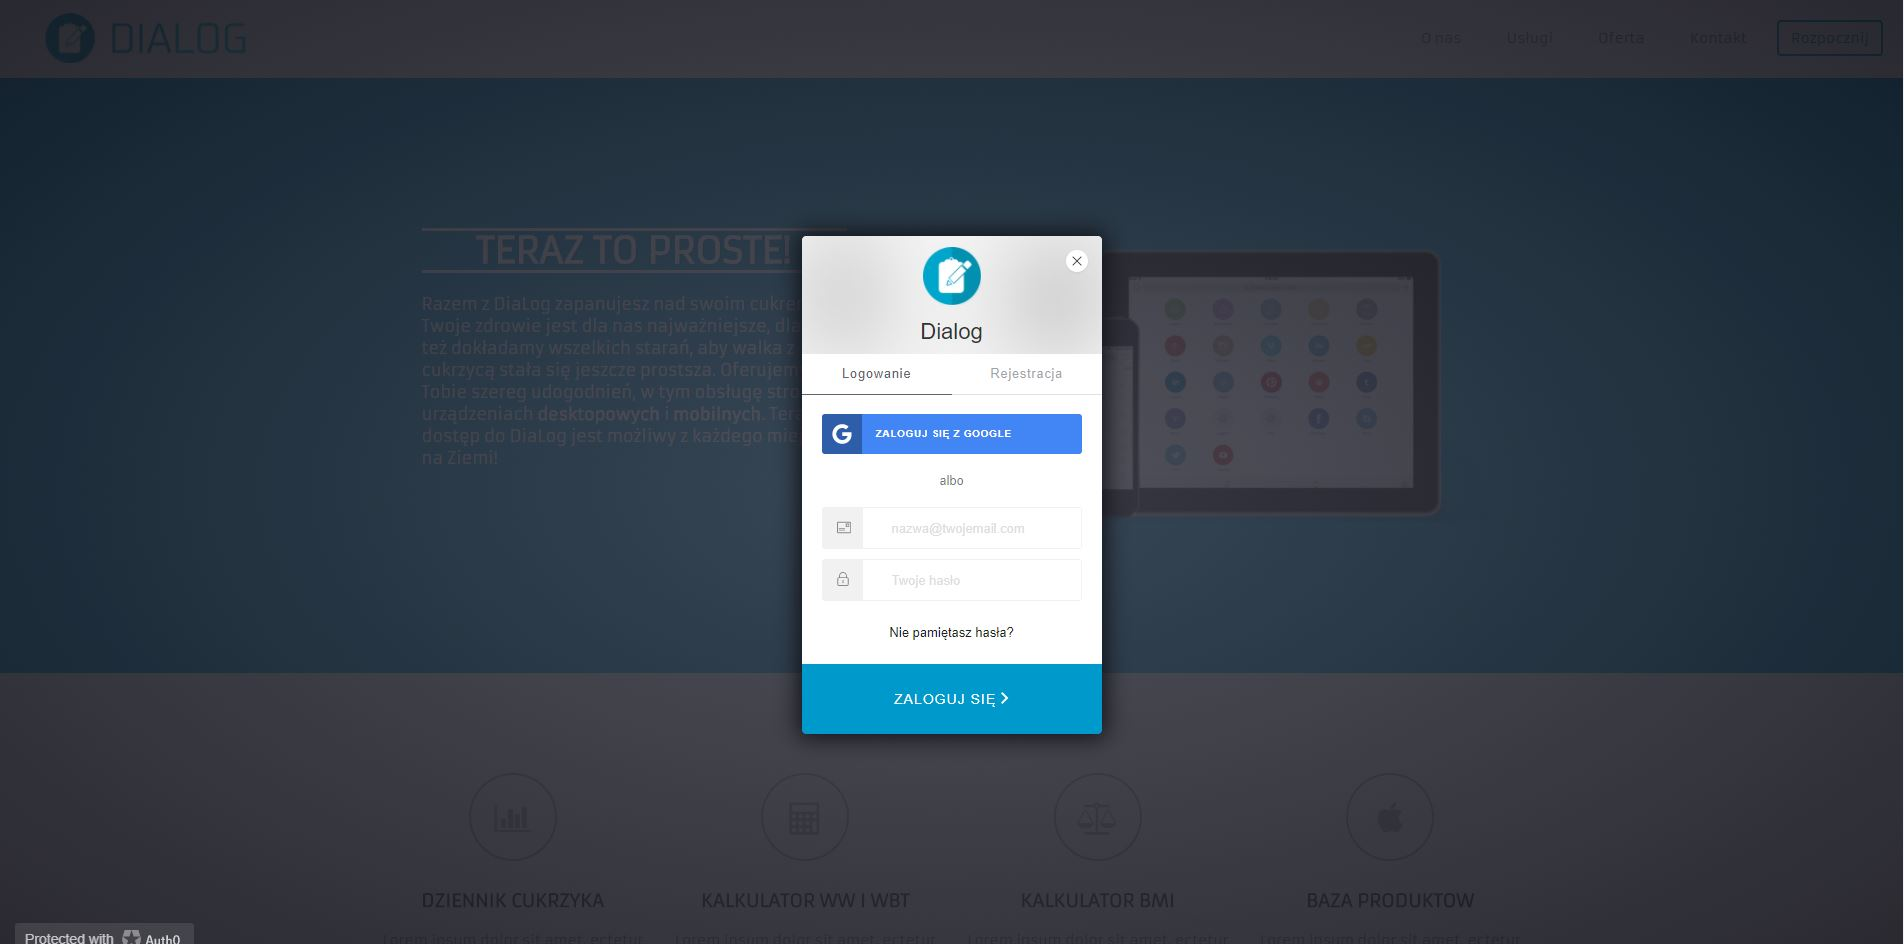
\includegraphics[scale=0.3]{images/logowanie_google.jpg}
	\caption{Okno logowania użytkownika}
	\label{Rys:logowanie}
\end{figure}

Po wpisaniu danych służących do logowania użytkownik uzyskuje dostęp do nowej pozycji w~ menu górnym -- \textit{Twój DiaLog}. Menu górne dostępne po zalogowaniu użytkownika zostało ukazane na rysunku  \ref{Rys:logged}.

\begin{figure}[h]
	\centering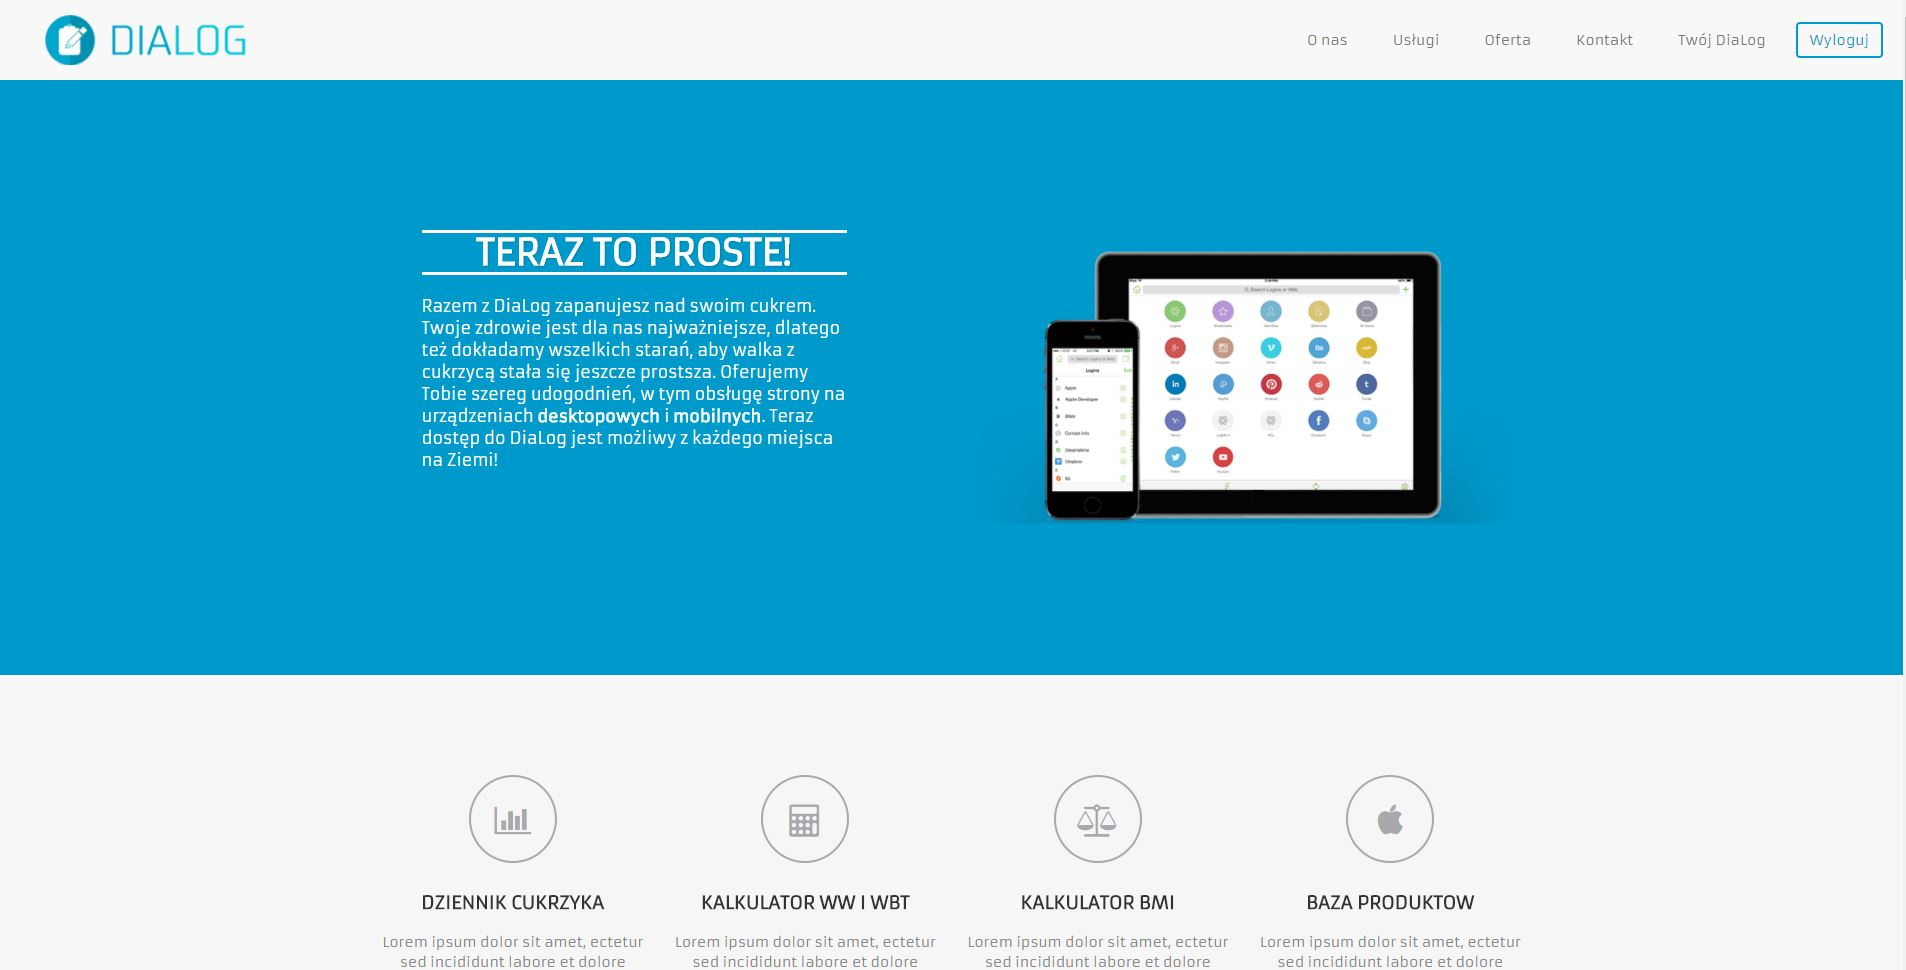
\includegraphics[scale=0.3]{images/ekran_logged.jpg}
	\caption{Menu górne rozszerzone o dodatkową pozycję -- \textit{Twój DiaLog}, dostępne po zalogowaniu użytkownika}
	\label{Rys:logged}
\end{figure}

\section{Użytkowanie panelu użytkownika zarejestrowanego}
Po uzyskaniu dostępu do zakładki \textit{Twój DiaLog} i kliknięciu jej, użytkownik uzyskuje dostęp do strony głównej panelu użytkownika zarejestrowanego będącej jednocześnie komponentem podsumowującym pomiary wprowadzone przez użytkownika. Początkowo, po rejestracji wykresy i tabela zestawień są puste, gdyż nie zawierają żadnych danych. Strona główna po kliknięciu pozycji górnego menu \textit{Twój DiaLog} została ukazana na rysunku \ref{Rys:firstPage}.

\begin{figure}[h]
	\centering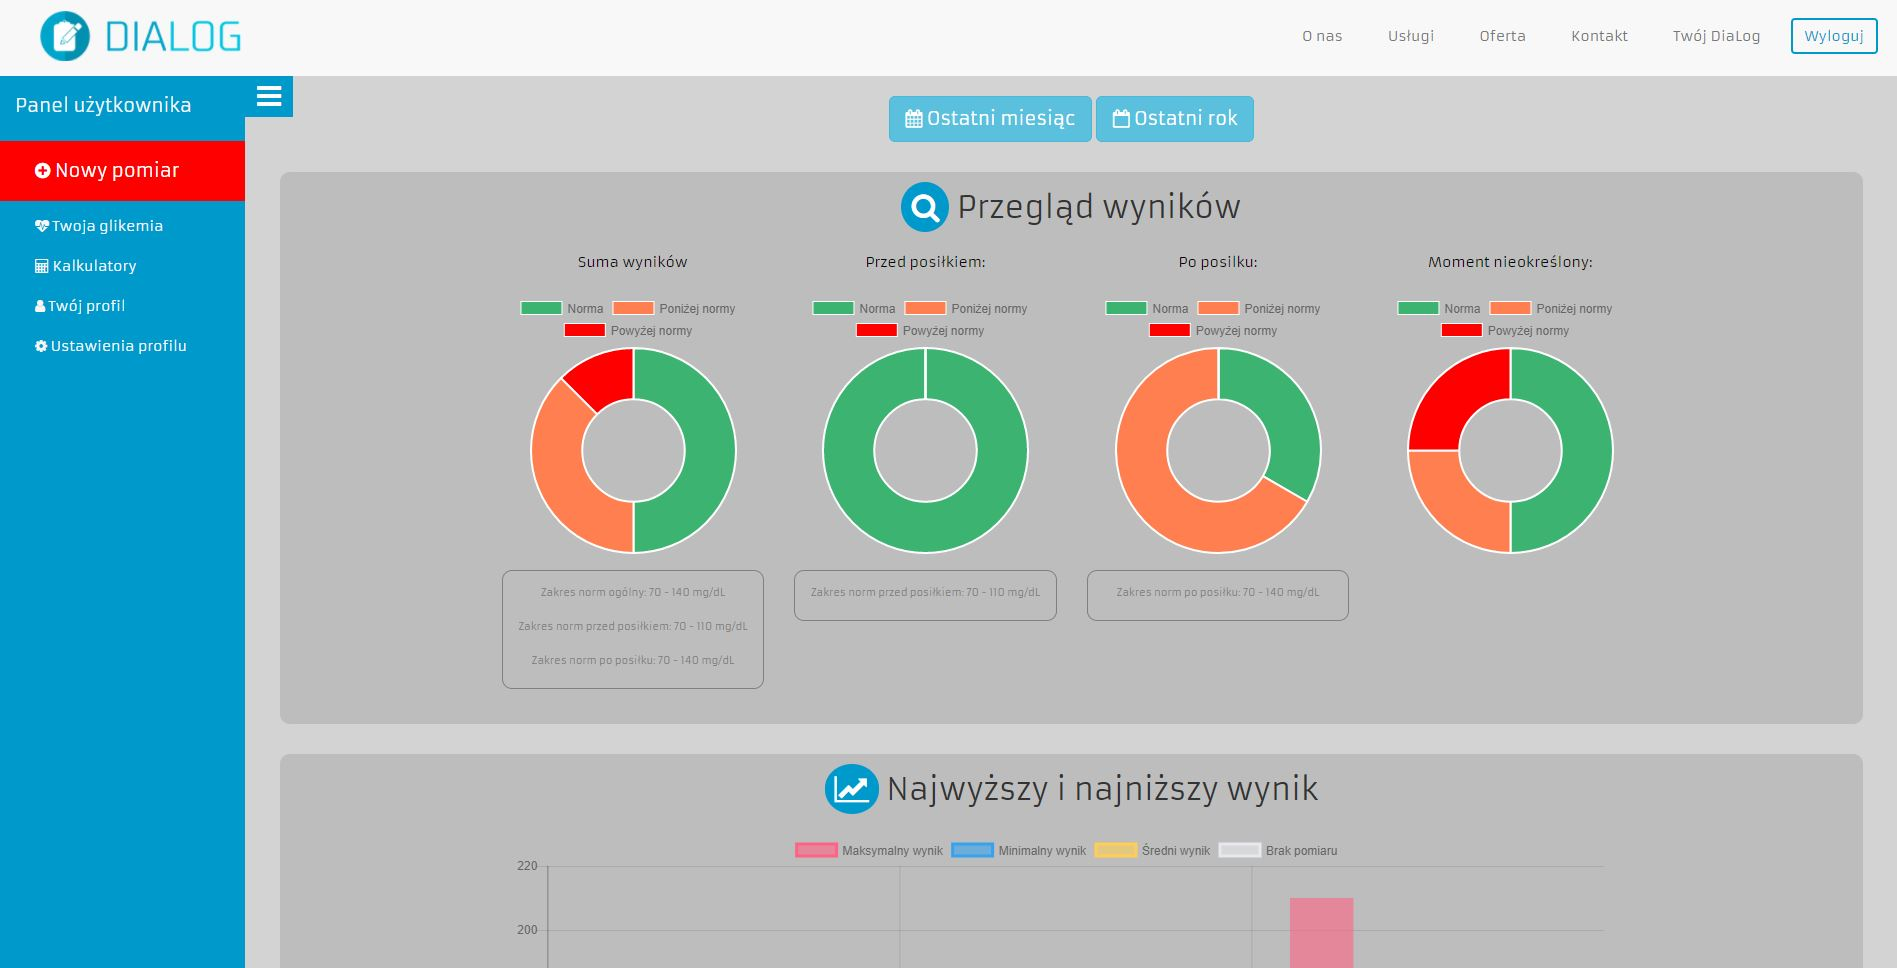
\includegraphics[scale=0.3]{images/first_page.jpg}
	\caption{Strona główna dostępna po kliknięciu przycisku menu górnego \textit{Twój DiaLog}, dostępnego po zalogowaniu użytkownika}
	\label{Rys:firstPage}
\end{figure}

\subsection{Twoja glikemia}
Zawartość dostępna z poziomu zakładki \textit{Twoja glikemia} wyświetlana jest jako strona główna po kliknięciu zakładki \textit{Twój DiaLog}. Zawiera ona wykresy kołowe podsumowujące ilość dodanych pomiarów glikemii. Każdy z czterech wykresów kołowych dotyczy odrębnego rodzaju pomiaru. Rodzaje pomiarów glikemii rozróżniane są w następujący sposób:

\begin{itemize}
	\item Przed posiłkiem,
	\item Po posiłku,
	\item Moment nieokreślony.
\end{itemize}

Pierwszy z wykresów jest sumą ilości pomiarów z pozostałych trzech wykresów. Ponadto, każdy z wykresów rozróżnia normy zakresu glikemii odpowiednie dla danego rodzaju pomiaru:

\begin{itemize}
	\item Przed posiłkiem:
	\begin{itemize}
		\item Norma ogólna: 70 - 140 mg/dL.
	\end{itemize}
	\item Po posiłku,
	\begin{itemize}
		\item Zakres norm przed posiłkiem: 70 - 110 mg/dL.
	\end{itemize}
	\item Moment nieokreślony.
	\begin{itemize}
		\item Zakres norm po posiłku: 70 - 140 mg/dL.
	\end{itemize}
\end{itemize}

Dla lepszej przejrzystości, do zaznaczenia norm na wykresie zostały użyte charakterystyczne kolory. Przy przekroczeniu normy wykres przyjmuje kolor czerwony. Jeżeli pomiar glikemii mieścił się w normie, wykres zostaje zaznaczony kolorem zielonym. W przypadku wartości glikemii znajdującej się poniżej normy wykres przyjmuje kolor pomarańczowy. Dodatkowo, po najechaniu kursorem na daną część wykresu użytkownikowi wyświetla się dymek z podpowiedzią ile pomiarów znajduje się w danym zakresie norm. 

\begin{figure}[h]
	\centering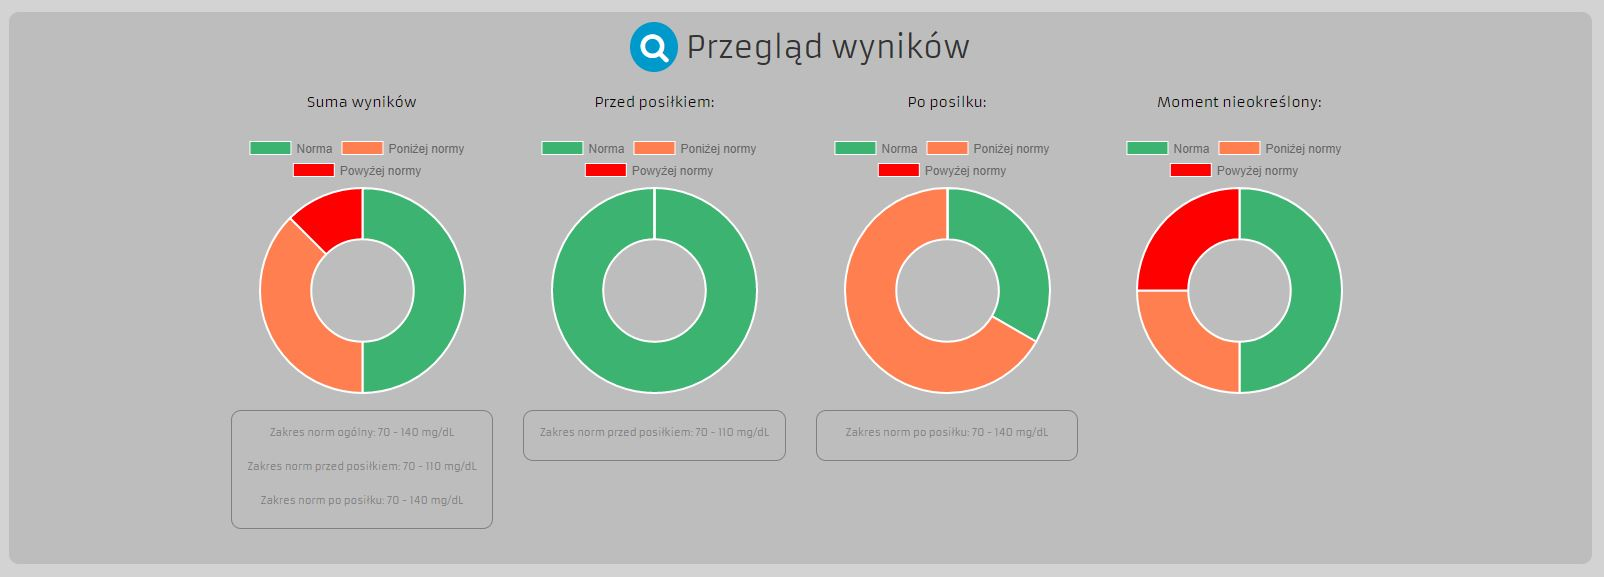
\includegraphics[scale=0.35]{images/bar_charts.jpg}
	\caption{Wykresy kołowe dostępne z poziomu zakładki \textit{Twoja glikemia}}.
	\label{Rys:barChart}
\end{figure}

Kolejnym elementem dostępnym z poziomu zakładki \textit{Twoja glikemia} są wykresy słupkowe. Zestawiają one maksymalny, minimalny oraz średni wynik dla każdego z rodzajów pomiarów glikemii. Po najechaniu na dany słupek wykresu użytkownik ma dostęp do informacji o wartości danego wyniku. 

\begin{figure}[h]
	\centering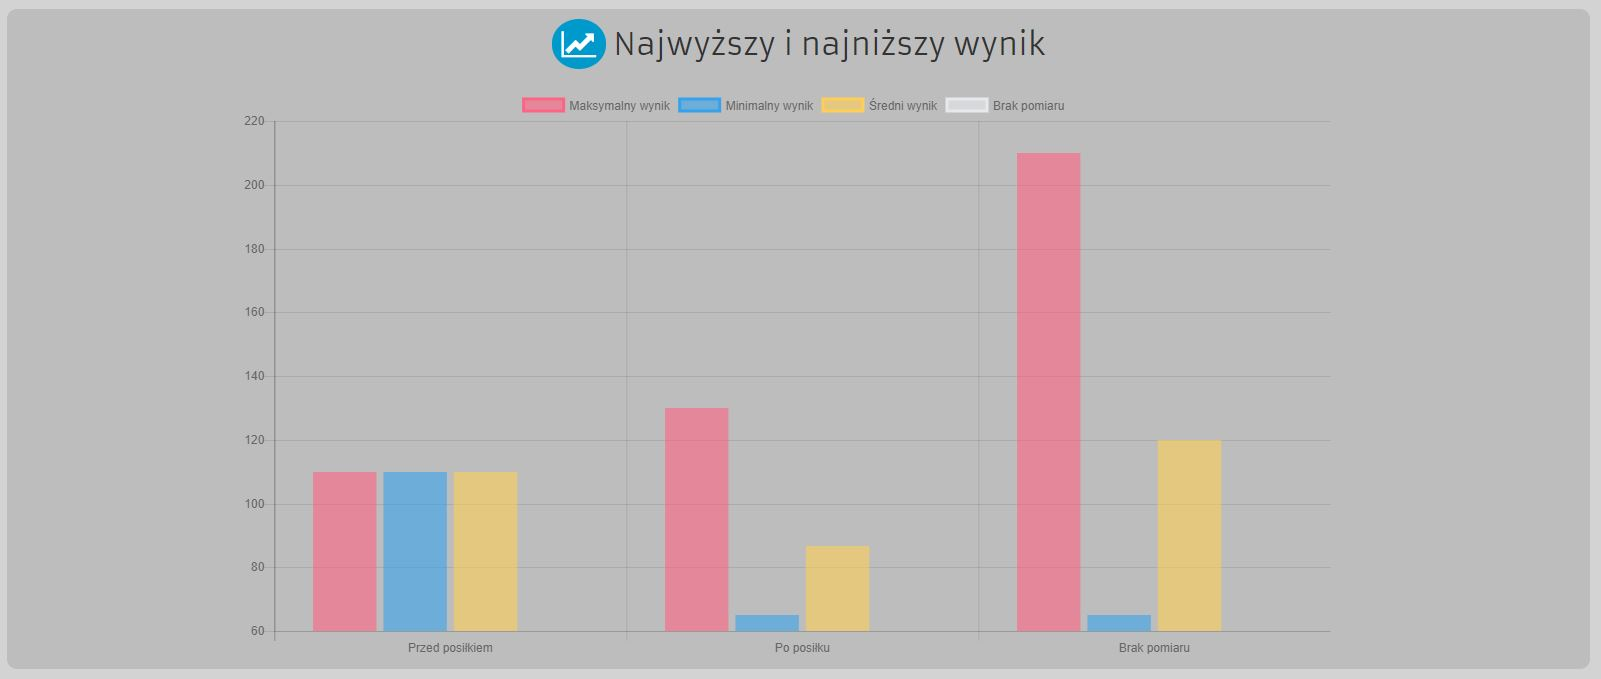
\includegraphics[scale=0.35]{images/normal_chart.jpg}
	\caption{Wykresy słupkowe dostępne z poziomu zakładki \textit{Twoja glikemia}}.
	\label{Rys:normalChart}
\end{figure}

Ostatnim z elementów zakładki \textit{Twoja glikemia} jest tabela zestawień. Podsumowuje ona (w~ zależności od pory dnia -- rano, południe, wieczór, noc) następujące dane: 

\begin{itemize}
	\item Liczba wyników, 
	\item Najwyższy wynik (mg/dL),
	\item Najniższy wynik (mg/dL),
	\item \% wyników powyżej normy,
	\item \% wyników poniżej normy,
	\item \% wyników w normie.
\end{itemize}

Ostatnia kolumna tabeli przedstawia sumę wyników danego wiersza. 

\begin{figure}[h]
	\centering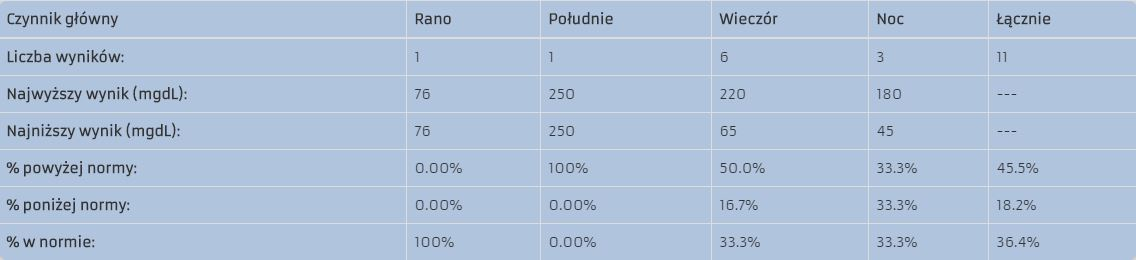
\includegraphics[scale=0.5]{images/table.jpg}
	\caption{Tabela zestawień pomiarów glikemii dostępna z poziomu zakładki \textit{Twoja glikemia}}.
	\label{Rys:table}
\end{figure}

Użytkownik ma możliwość wybrania przedziału czasu, na podstawie którego wyświetlane mają być dane. Dostępne są dwie opcje -- \textit{Ostatni miesiąc} oraz \textit{Ostatni rok}. Wyboru dokonuje się poprzez kliknięcie jednego z dwóch dostępnych przycisków na szczycie podstrony.

\newpage

\subsection{Dodaj pomiar}
Zakładka \textit{Dodaj pomiar} otwiera okno modalne dodawania nowego pomiaru (rys. \ref{Rys:measurement}). Z poziomu tego okna użytkownik wprowadza dane, które zestawiane są później na stronie komponentu \textit{Twoja glikemia} w postaci wykresów i tabeli zestawień:

\begin{itemize}
	\item Data i godzina pomiaru,
	\item Wartość glikemii,
	\item Moment pomiaru,
	\item Krótka notatka.
\end{itemize}
Po naciśnięciu przycisku \textit{Dodaj} zostaje dodany do bazy danych pomiarów nowy pomiar.  

\begin{figure}[h]
	\centering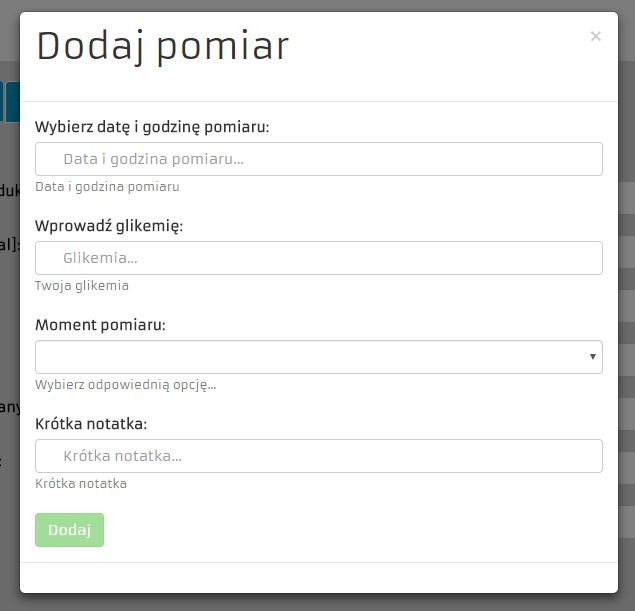
\includegraphics[scale=0.5]{images/measurement.jpg}
	\caption{Okno modalne dodawania nowego pomiaru}
	\label{Rys:measurement}
\end{figure}

\subsection{Kalkulatory}
Zakładka \textit{Kalkulatory} pozwala użytkownikowi na uzyskanie dostępu do kalkulatora \textit{BMI (Body Mass Index)} oraz do kalkulatora wymienników węglowodanowych oraz białkowo~-tłuszczowych, dostępnego wraz z tabelą makroskładników produktów spożywczych pochodzących z bazy danych produktów. 
Kalkulator \textit{BMI (Body Mass Index)} pozwala obliczyć współczynnik masy do wzrostu. Składa się on z dwóch pól typu 
\textit{Input}. W pierwszym z~ nich użytkownik wpisuje swoją wagę, a~ w następnym wzrost (rys. \ref{Rys:bmiBefore}). Po~ kliknięciu przycisku \textit{Oblicz} użytkownik otrzymuje informację o uzyskanym wyniku współczynnika \textit{BMI} oraz podpowiedź do jakiej grupy osób (ze względu na wagę) się zalicza (rys. \ref{Rys:bmiAfter}):

\begin{itemize}
	\item osoby z niedowagą,
	\item osoby z wagą prawidłową,
	\item osoby z nadwagą,
	\item osoby z otyłością I stopnia,
	\item osoby z otyłością II stopnia,
	\item osoby z otyłością III stopnia.
\end{itemize}

\begin{figure}[h]
	\centering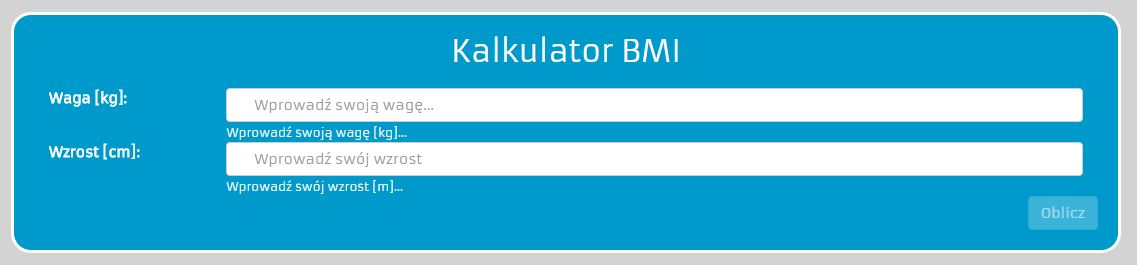
\includegraphics[scale=0.5]{images/bmi_before.jpg}
	\caption{Interfejs kalkulatora BMI}.
	\label{Rys:bmiBefore}
\end{figure}

\begin{figure}[h]
	\centering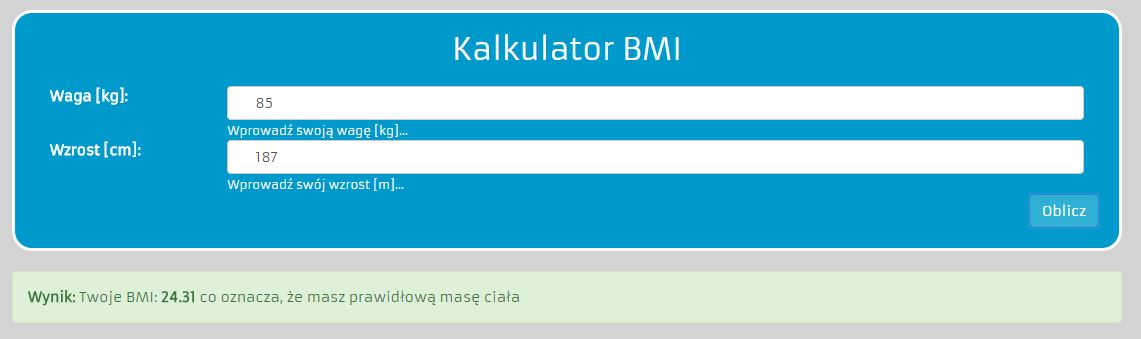
\includegraphics[scale=0.5]{images/bmi_after.jpg}
	\caption{Interfejs kalkulatora BMI po uzyskaniu wyniku}.
	\label{Rys:bmiAfter}
\end{figure}

Kolejną funkcjonalnością dostępną z poziomu zakładki \textit{Kalkulatory} menu bocznego jest kalkulator wymienników węglowodanowych i wymienników białkowo-tłuszczowych na podstawie tabeli makroskładników produktów dostępnych z poziomu tabeli \textit{products}, która może być stale rozszerzana przez zalogowanych użytkowników aplikacji (rys. \ref{Rys:wwBefore}). Wynik przedstawiany jest w postaci kolumn dołączonych do tabeli makroskładników danego produktu. Aby obliczyć wartość wymienników węglodowanowych i wymienników białkowo-tłuszczowych należy wybrać dany produkt poprzez wpisanie ciągu (bądź części ciągu) znaków w polu formularza o nazwie \textit{Wybierz produkt}. Do tego pola przypięty jest inteligentny moduł wyszukiwania znajdujący produkty po słowach kluczowych. Po wpisaniu części wyrazu moduł podpowiada użytkownikowi najbardziej prawdopodobne wyniki w~ postaci listy rozwijanej. Dodatkowo użytkownik ma możliwość podania porcji produktu w polu \textit{Wpisz wagę produktu [g]}. Wartości makroskładników i wyników obliczonych przez kalkulatory są wówczas dynamicznie zmieniane w zależności od wpisanej porcji produktu. Domyślna wartość pola to 100 [g]. 

Dodatkowo, jako ostatnia kolumna tabeli dodana została informacja czy produkt może być szkodliwy dla zdrowia osoby chorej na cukrzycę czy też nie. System rekomendacji oparty jest na ilości węglowodanów zawartych w produkcie. Jeżeli w 100 gramach produktu, 50 gram to węglowodany, wówczas produkt może okazać się szkodliwy w diecie cukrzyka (rys. \ref{Rys:wwAfter}). 

\begin{figure}[h]
	\centering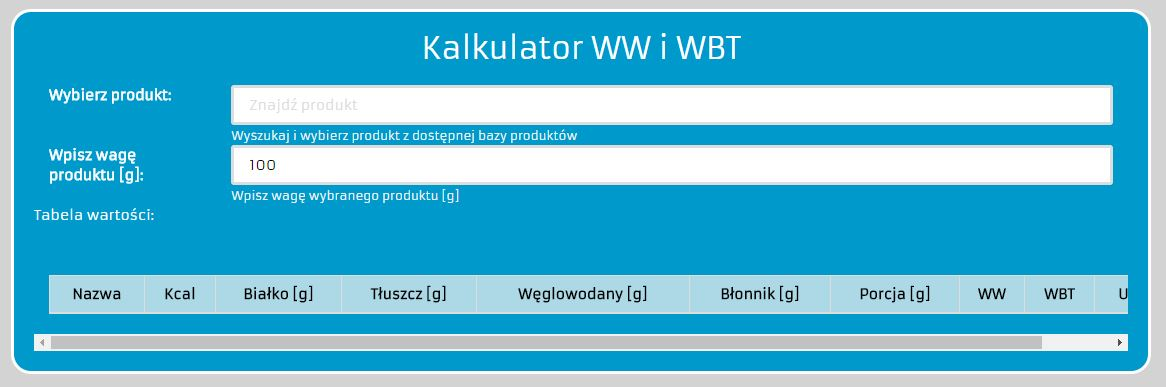
\includegraphics[scale=0.5]{images/ww_before.jpg}
	\caption{Interfejs kalkulatora wymienników węglowodanowych i~ białkowo-tłuszczowych}.
	\label{Rys:wwBefore}
\end{figure}

\begin{figure}[h]
	\centering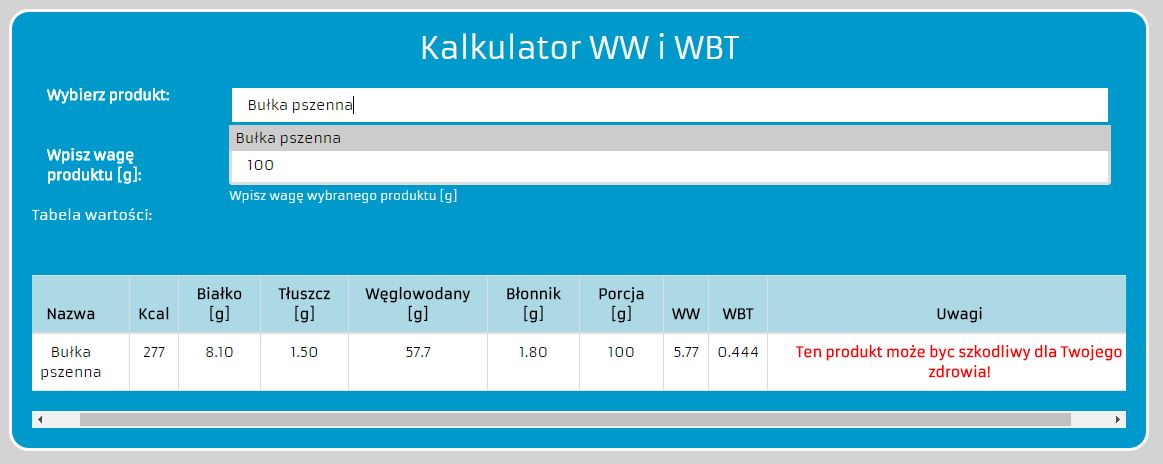
\includegraphics[scale=0.5]{images/ww_after.jpg}
	\caption{Interfejs kalkulatora wymienników węglowodanowych i~ białkowo-tłuszczowych po uzyskaniu wyniku}.
	\label{Rys:wwAfter}
\end{figure}

\newpage

Użytkownik zarejestrowany ma również możliwość dodawania produktów do bazy danych produktów. Formularz dodawania nowego produktu dostępny jest również z poziomu zakładki \textit{Twoja glikemia} -- karta \textit{Dodaj produkt} (rys. \ref{Rys:addProduct}). 

\begin{figure}[h]
	\centering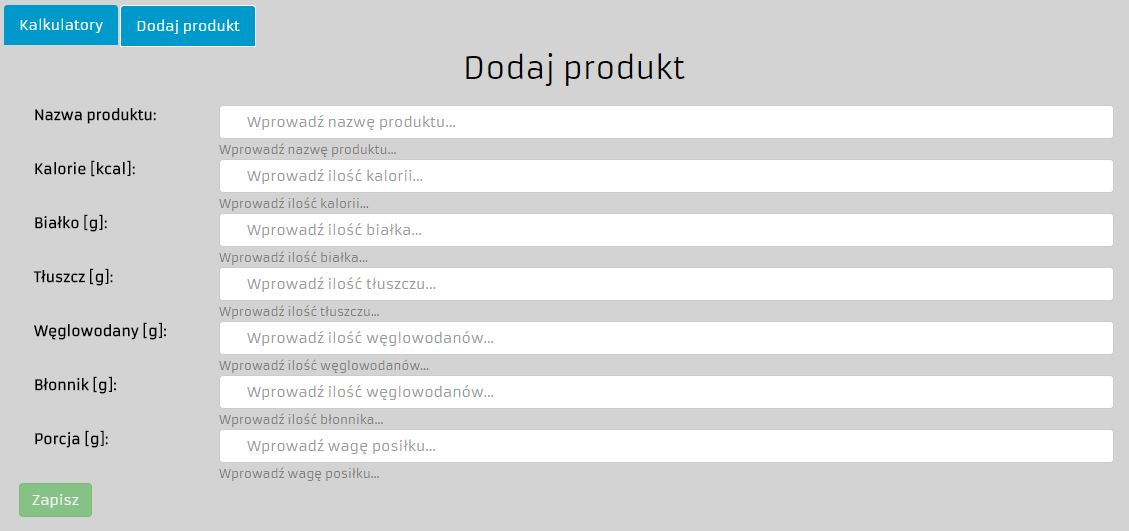
\includegraphics[scale=0.5]{images/add_product.jpg}
	\caption{Formularz dodawania nowego produktu}.
	\label{Rys:addProduct}
\end{figure}

Po wypełnieniu wszystkich pól: 
\begin{itemize}
	\item Nazwa produktu,
	\item Kalorie [kcal],
	\item Białko [g],
	\item Tłuszcz [g],
	\item Węglowodany [g],
	\item Błonnik [g],
	\item Porcja [g]
\end{itemize}
produkt jest dynamicznie dodawany do bazy danych i bezpośrednio dostępny z pozycji modułu kalkulatora do obliczania wymienników węglowodanowych i białkowo-tłuszczowych.

\subsection{Twój profil}
Z poziomu zakładki \textit{Twój profil} użytkownik ma możliwość dodania informacji zarówno o profilu (rys. \ref{Rys:yourProfile}) jak i danych medycznych (rys. \ref{Rys:medicalData}). Czynność ta odbywa się przy pomocy dwóch formularzy z odpowiednimi polami:

\begin{itemize}
	\item Dla karty \textit{Twój profil}
	\begin{itemize}
		\item imię,
		\item nazwisko,
		\item PESEL,
		\item opiekun -- lista rozwijana,
		\item ulica,
		\item nr domu,
		\item miasto,
		\item kod pocztowy,
		\item numer telefonu,
		\item aktualny glukometr -- lista rozwijana,
		\item poprzedni glukometr -- lista rozwijana,
		\item numer seryjny glukometru.
	\end{itemize}
	\item Dla karty \textit{Dane medyczne}
	\begin{itemize}
		\item typ cukrzycy -- lista rozwijana,
		\item rok zachorowania -- lista rozwijana,
		\item rodzaj insuliny -- lista rozwijana,
		\item przyjmowany lek -- lista rozwijana,
		\item inne leki i insuliny,
		\item BMI,
		\item wzrost,
		\item waga,
		\item hBA1c.
	\end{itemize}
\end{itemize}

Przy pierwszym wpisaniu danych do wszystkich pól formularza i zatwierdzeniu ich przyciskiem \textit{Zapisz}, zostanie wykonana operacja zapisania danych do obydwu tabel bazy danych. Przy każdorazowym otwarciu zakładki \textit{Twój profil} dane te będą czytane z bazy danych do pól formularza. W~ przypadku chęci zaktualizowania informacji użytkownik nadpisuje pola formularza nowymi danymi i wykonywana jest operacja \textit{UPDATE} zarówno w przypadku jednej, jak i drugiej tabeli.

\begin{figure}[h]
	\centering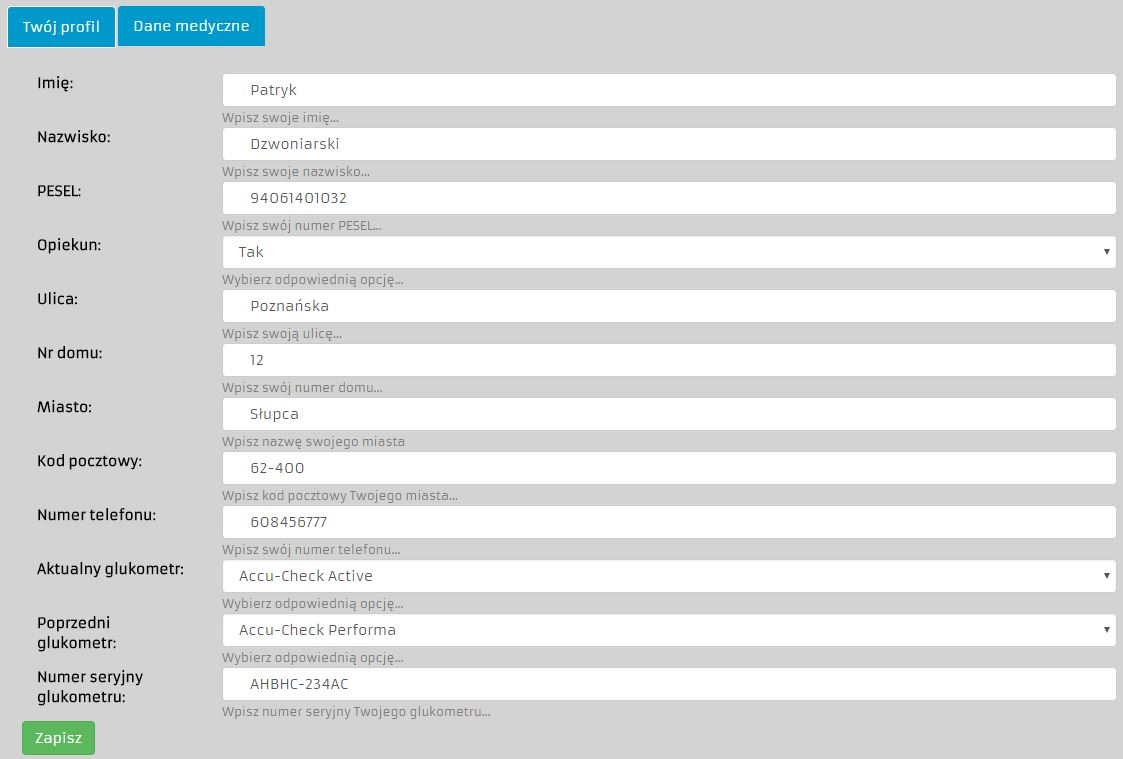
\includegraphics[scale=0.5]{images/yourprofile.jpg}
	\caption{Formularz dodawania i aktualizacji informacji o profilu}
	\label{Rys:yourProfile}
\end{figure}

\newpage

\begin{figure}[h]
	\centering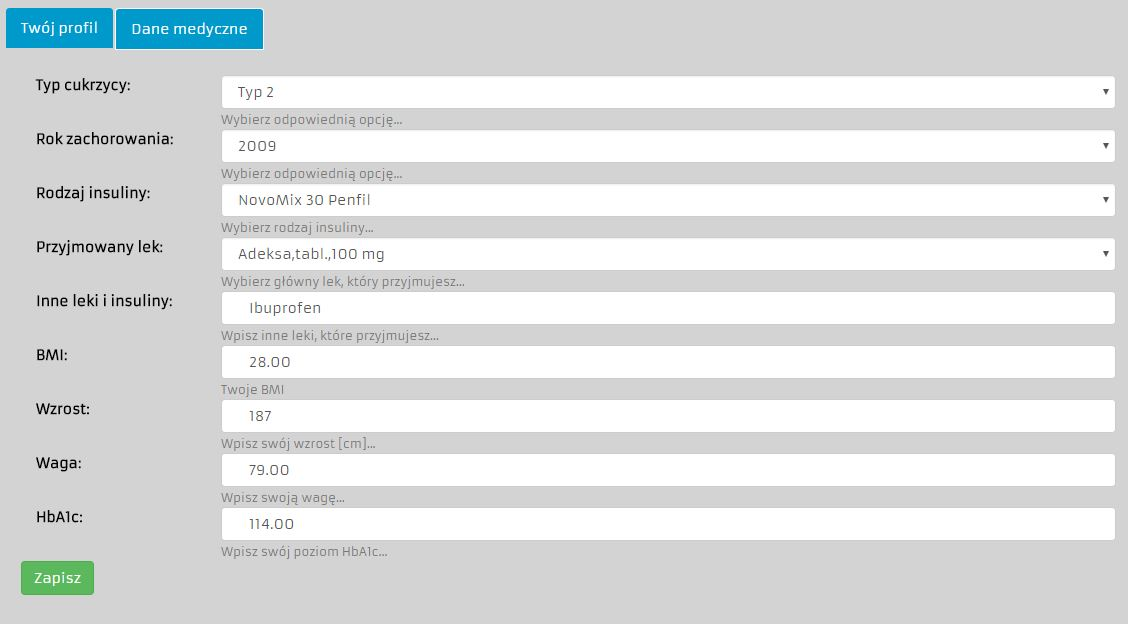
\includegraphics[scale=0.5]{images/medical_data.jpg}
	\caption{Formularz dodawania i aktualizacji danych medycznych użytkownika profilu}
	\label{Rys:medicalData}
\end{figure}

\subsection{Ustawienia profilu}
W zakładce \textit{Ustawienia profilu} użytkownik ma możliwość dodania, bądź zaktualizowania bieżących zakresów glikemii (rys. \ref{Rys:profileSettings}). Komponent składa się z trzech pól formularza:

\begin{itemize}
	\item Hipoglikemia, 
	\item Hiperglikemia,
	\item Hiperglikemia po posiłku.
\end{itemize}

\begin{figure}[h]
	\centering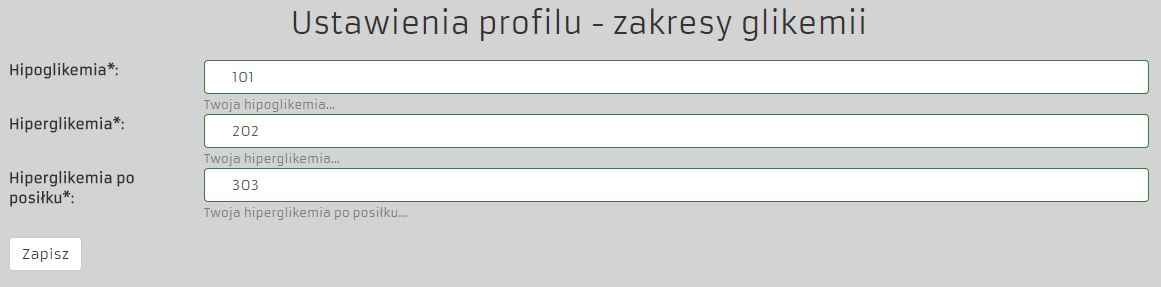
\includegraphics[scale=0.5]{images/profile_settings.jpg}
	\caption{Formularz dodawania i aktualizacji danych dotyczących zakresów glikemii użytkownika}
	\label{Rys:profileSettings}
\end{figure}


Każde pole może być w dowolnym czasie aktualizowanie (operacja \textit{UPDATE}) w bazie danych. Ponadto dane wczytywane są bezpośrednio do pól formularza przy użyciu metody \textit{GET}. 